% !TeX program = xelatex
% !TeX encoding = UTF-8
% !TeX spellcheck = en_US
% !BIB program = biber
%% 
%% The above lines help editors like TeXstudio to automatically choose the right tools
%% to compile your LaTeX source file. If your tool does not support these magic comments,
%% you will need to make appropriate manual choices.
%% 
%% You can safely use "pdflatex" instead of "xelatex" if you prefer the pdfLaTeX toolchain.
%% However, pdfLaTeX will not be able to deliver the professional font experience that you
%% will get with XeLaTeX. You can also safely use "lualatex" instead of "xelatex" while
%% preserving the professional font experience if you prefer the LuaLaTeX toolchain.
%% 
%% _Important_: These magic comments should be on the first lines of your source file.
%% 
%%%%%%%%%%%%%%%%%%%%%%%%%%%%%%%%%%%%%%%%%%%%%%%%%%%%%%%%%%%%%%%%%%%%%%%%%%%%%%%%

%%%%%%%%%%%%%%%%%%%%%%%%%%%%%%%%%%%%%%%%%%%%%%%%%%%%%%%%%%%%%%%%%%%%%%%%%%%%%%%%
%% 
%%            JJJJ   K                         K   UUUU         UUUU  
%%            JJJJ   KKKK                   KKKK   UUUU         UUUU  
%%            JJJJ   KKKKKK               KKKKKK   UUUU         UUUU  
%%            JJJJ      KKKKKK         KKKKKK      UUUU         UUUU  
%%            JJJJ         KKKKKK   KKKKKK         UUUU         UUUU  
%%            JJJJ            KKKKKKKKK            UUUU         UUUU  
%%    JJ     JJJJJ               KKK               UUUUU       UUUUU  
%%  JJJJJJJJJJJJJ    KKKKKKKKKKKKKKKKKKKKKKKKKKK    UUUUUUUUUUUUUUU   
%%    JJJJJJJJJ      KKKKKKKKKKKKKKKKKKKKKKKKKKK      UUUUUUUUUUU     
%% 
%% This is an example file for using the JKU LaTeX technical report template
%% for your seminar report.
%% 
%% Template created by Michael Roland (2023)
%% 
%%%%%%%%%%%%%%%%%%%%%%%%%%%%%%%%%%%%%%%%%%%%%%%%%%%%%%%%%%%%%%%%%%%%%%%%%%%%%%%%

%%%%%%%%%%%%%%%%%%%%%%%%%%%%%%%%%%%%%%%%%%%%%%%%%%%%%%%%%%%%%%%%%%%%%%%%%%%%%%%%
%% 
%% Document class: This is a koma-script article.
%% 
\documentclass[a4paper,oneside,10pt,english]{scrartcl}
%% 
%% The comma-separated list in square brackets are class options.
%% Useful options that you might want to use:
%% 
%% Paper size:
%%  * a4paper ... A4 paper size
%% 
%% Optimize for single-sided or double-sided printing:
%%  * oneside ... single-sided
%%  * twoside ... double-sided
%% 
%% Base font size:
%%  * 10pt ... 10-pt font is used for normal text
%%  * 11pt ... 11-pt font is used for normal text
%% 
%% Define document languages (the last specified language becomes the document default
%% language):
%%  * ngerman ... German
%%  * english ... English
%%  * ...
%% 
%% Alternate document classes: The JKU report template supports the koma-script classes
%% `scrartcl', `scrreprt' and `scrbook'. The article class `scrartcl' is well-suited
%% for a typical seminar report. However, `scrbook' or `scrreprt' may be better
%% suited for longer reports since they permit structuring your work in chapters.
%%  
%% _Important_: The document class should be the first line of LaTeX code in your main
%% source file. Do not place anything but comments / magic comments above that line (unless
%% you really know what you are doing).
%% 
%%%%%%%%%%%%%%%%%%%%%%%%%%%%%%%%%%%%%%%%%%%%%%%%%%%%%%%%%%%%%%%%%%%%%%%%%%%%%%%%

%%%%%%%%%%%%%%%%%%%%%%%%%%%%%%%%%%%%%%%%%%%%%%%%%%%%%%%%%%%%%%%%%%%%%%%%%%%%%%%%
%% 
%% Treat input files as UTF-8 encoded. Make sure to always load this when you use pdfLaTeX
%% so that pdfLaTeX knows how to read and interpret characters in this source file.
%% 
\usepackage[utf8]{inputenc}
%% 
%%%%%%%%%%%%%%%%%%%%%%%%%%%%%%%%%%%%%%%%%%%%%%%%%%%%%%%%%%%%%%%%%%%%%%%%%%%%%%%%

%%%%%%%%%%%%%%%%%%%%%%%%%%%%%%%%%%%%%%%%%%%%%%%%%%%%%%%%%%%%%%%%%%%%%%%%%%%%%%%%
%% 
%% Use the JKU LaTeX technical report template for this document.
%% 
\usepackage[seminarreport,fancyfonts]{jkureport}
%% 
%% The comma-separated list in square brackets are theme options. Useful options that you
%% might want to use:
%% 
%% Document type:
%%  * phdthesis     ... PhD thesis.
%%  * mathesis      ... Master's thesis.
%%  * diplomathesis ... Diploma thesis.
%%  * bathesis      ... Bachelor's thesis.
%%  * seminarreport ... Seminar report.
%%  * techreport    ... Technical report.
%% 
%% Color scheme selection options:
%%  * JKU  ... Use JKU (gray) color scheme (this is the default if no scheme is selected).
%%  * BUS  ... Use Business School color scheme.
%%  * LIT  ... Use Linz Institute of Technology color scheme.
%%  * MED  ... Use MED faculty color scheme.
%%  * RE   ... Use RE faculty color scheme.
%%  * SOE  ... Use School of Education color scheme.
%%  * SOWI ... Use SOWI faculty color scheme.
%%  * TNF  ... Use TNF faculty color scheme.
%% 
%% Space-efficient monospace font options (requires XeTeX/LuaTeX):
%%  * compactmono   ... Use condensed fixed-width font everywhere.
%%  * nocompactverb ... Do not use condensed fixed-width font for verbatim and listings.
%% 
%% Style-breaking options:
%%  * noimprint      ... Do not insert imprint on title pages.
%%  * nojkulogo      ... Do not insert JKU & K logos on title pages.
%%  * capstitle      ... Set document title in capital letters.
%%  * nofancyfonts   ... Do not use custom TTF fonts with XeTeX/LuaTeX / supress pdfLaTeX warning.
%%  * equalmargins   ... Decrease the outer page margin to have both page margins of equal size
%%                       (the additional outer margin is intentional and to be used for
%%                       anotations; equalmargins also causes the text width to be
%%                       significantly larger than optimal for reading).
%% 
%% Experimental options:
%%  * mathastext ... Use standard document fonts (enhanced with symbols from Fira Math font
%%                   when using XeTeX/LuaTeX) in math mode.
%% 
%% Advanced options:
%%  * noautopdfinfo     ... Do not automatically try to add pdfinfo with hyperref from document
%%                          metadata fields.
%%  * logopath={<path>} ... Set the path where the theme can find its own logo resources. This
%%                          should typically be a relative path and the default is `./logos'.
%%  * fontpath={<path>} ... Set the path where the theme can find its own font resources. This
%%                          should typically be a relative path and the default is `./fonts'.
%% 
%% Hint: Boolean options can be used in the forms `option' or `option=true' the enable the
%% option and `nooption' or `option=false' to disable the option.
%% 
%%%%%%%%%%%%%%%%%%%%%%%%%%%%%%%%%%%%%%%%%%%%%%%%%%%%%%%%%%%%%%%%%%%%%%%%%%%%%%%%

%%%%%%%%%%%%%%%%%%%%%%%%%%%%%%%%%%%%%%%%%%%%%%%%%%%%%%%%%%%%%%%%%%%%%%%%%%%%%%%%
%% 
%% This is the place where you can load additional packages. If you want to load
%% a package `biblatex', you would use the command `\usepackage{biblatex}'.
%% 

\usepackage{csquotes}
\usepackage[backend=biber,citestyle=numeric,sortcites=true,maxcitenames=2,style=ACM-Reference-Format]{biblatex}
\setcounter{biburlnumpenalty}{100} %% reducing biburl* penalties typically improves URL placement in bibliography
\setcounter{biburllcpenalty}{100}
\setcounter{biburlucpenalty}{100}
\usepackage{todonotes}
\usepackage{import}
\usepackage{amsfonts}
\usepackage{subfigure}
\usepackage{acronym}

%% 
%%%%%%%%%%%%%%%%%%%%%%%%%%%%%%%%%%%%%%%%%%%%%%%%%%%%%%%%%%%%%%%%%%%%%%%%%%%%%%%%

%%%%%%%%%%%%%%%%%%%%%%%%%%%%%%%%%%%%%%%%%%%%%%%%%%%%%%%%%%%%%%%%%%%%%%%%%%%%%%%%
%% 
%% Bibliography data files.
%% 

\addbibresource{references.bib}

%% 
%%%%%%%%%%%%%%%%%%%%%%%%%%%%%%%%%%%%%%%%%%%%%%%%%%%%%%%%%%%%%%%%%%%%%%%%%%%%%%%%

\begin{document}
%%%%%%%%%%%%%%%%%%%%%%%%%%%%%%%%%%%%%%%%%%%%%%%%%%%%%%%%%%%%%%%%%%%%%%%%%%%%%%%%
%% 
%% Report information and title page
%% 

%% Command \title{title}: sets the title of your report
\title{Weight-sparse transformers are interpretable: a report}

%% Command \titleshort{short title}: sets an abbreviated version of the report title for page heads
%\titleshort{Optional space for your abbreviated title}

%% Command \subtitle{subtitle}: sets the subtitle for seminar/technical reports (not used for theses)
\subtitle{Seminar Report}

%% Command \author{name}: sets the author's name; use \prefix{} and \suffix{} to add academic titles
%%   and suffixes, use \matno{} to add the immatriculation number
\author{\prefix{} Ivor~Štúr \suffix{}\matno{12416055}}

%% Command \supervisor[number,gender]{name}: sets the name of the supervisor (where number optionally
%%   defines the rank of the supervisor (1-3) and gender specifies if the supervisor is male or female
%%   to adapt gener-specific terms in German)
\supervisor[1]{\prefix{Prof. Dr.} Maximilian~Plattner}
%\supervisor[2]{\prefix{Prof. Dr.} Firstname~Lastname}

%% Command \submissiondepartment{institute or department}: set the course or department that the thesis
%%   is submitted at
\submissiondepartment{Institute of Machine Learning: Seminar in AI}

%% Command \date{YYYY-MM-DD}: set the day of submission (defaults to today)
%\date{2020-04-09}

%% Command \abstract{text}: set the document abstract on the title page
\abstract{Weight-sparse transformers have interpretable circuits}

%% Command \keywords{text}: set the document keywords
%\keywords{Space for your comma-separated keywords}


%% Finally, print the title page using the above information:
\maketitle
%% 
%%%%%%%%%%%%%%%%%%%%%%%%%%%%%%%%%%%%%%%%%%%%%%%%%%%%%%%%%%%%%%%%%%%%%%%%%%%%%%%%

%%%%%%%%%%%%%%%%%%%%%%%%%%%%%%%%%%%%%%%%%%%%%%%%%%%%%%%%%%%%%%%%%%%%%%%%%%%%%%%%
%% 
%% Add a table of contents
%% 

%% Make sure to start the table of contents on a new odd page (odd is only relevant in twoside layout)
\cleardoubleoddpage
%% Print the table of contents
\tableofcontents

%% Make sure to start the list of acronyms on a new odd page (odd is only relevant in twoside layout)
%\cleardoubleoddpage
%% Include list of acronyms (optional and often not necessary)
%\import{./}{acronyms}

%% 
%%%%%%%%%%%%%%%%%%%%%%%%%%%%%%%%%%%%%%%%%%%%%%%%%%%%%%%%%%%%%%%%%%%%%%%%%%%%%%%%

%%%%%%%%%%%%%%%%%%%%%%%%%%%%%%%%%%%%%%%%%%%%%%%%%%%%%%%%%%%%%%%%%%%%%%%%%%%%%%%%
%% 
%% Abstract: Instead of an abstract on the title page (see \abstract{...}), you
%% sometimes want to add an abstract as its own unnumbered section.
%% 

%% (Optionally) let the abstract start on a new odd page (odd is only relevant in twoside layout)
% \cleardoubleoddpage

% \addsec{Abstract}

% Space for your abstract.


%% 
%%%%%%%%%%%%%%%%%%%%%%%%%%%%%%%%%%%%%%%%%%%%%%%%%%%%%%%%%%%%%%%%%%%%%%%%%%%%%%%%

%%%%%%%%%%%%%%%%%%%%%%%%%%%%%%%%%%%%%%%%%%%%%%%%%%%%%%%%%%%%%%%%%%%%%%%%%%%%%%%%
%% 
%% Add your report sections ...
%% 

%% (Optionally) let the main sections start on a new odd page (odd is only relevant in twoside layout)
\cleardoubleoddpage

\section{Introduction}
\label{sec:introduction}

Despite the rapid increase in the capabilities of large language models, namely transformers, these architectures are not human-interpretable. Mechanistic interpretability seeks to reverse engineer these networks, but neural activations and weights are typically not comprehensible to humans. \par 
The paper \textcite{gao2025weightsparsetransformersinterpretablecircuits} proposes using weight-sparse transformers to achieve human-interpretable circuits. Training such sparse models requires them  to be trained \textit{de novo}, which is not effective and unlikely to match their dense counterparts. In addition, the paper shows results suggesting that their method can also be adapted to explain existing dense models. \par
Findings show that sometimes neuron activations often correspond to simple concepts and the resulting prediction may be intuitive. 

\section{Methodology}
\label{sec:methodology}

The main objective is to construct Transformer models that are "interpretable by design" through the enforcement of weight sparsity. Unlike post-hoc interpretability methods that attempt to explain dense models, this approach integrates structural constraints directly into the training loop to ensure that the resulting circuits are sparse, localized, and human-understandable. The models were evaluated on simple tasks to choose between one of two options, for example quote detector.

\subsection{Sparse weight enforcement}

The primary departure from standard training is the enforcement of a strict $L_0$ constraint on the weight matrices, which sets most, except the largest weights to zero. 
\begin{itemize}
  \item \textbf{Magnitude-Based Sparsity:} Sparsity is not induced via a penalty term (like $L_1$ norm) but is enforced as a hard constraint during optimization. After every AdamW \textcite{loshchilov2019decoupledweightdecayregularization} optimization step, only the $k$ weights with the largest absolute magnitudes in each weight matrix and bias vector are retained, while all other parameters are set to zero.
  \item \textbf{Scaling Width with Fixed Parameters:} This method allows to scale the model's width (hidden dimension and number of heads) while keeping the total number of non-zero parameters ($N_{nz}$) constant.
\end{itemize}

\subsection{Training and optimization}

The models are pretrained de novo, using AdamW optimizer. Weights are initialized using standard techniques, but the sparsity mask is dynamic and evolves throughout the training process.

\subsection{Interpretability measure}

Measured on 20 manually constructed python code binary tasks, for example to predict whether to close a string with a single or double quote, where the resulting label depends only on the context. \par

The model is further pruned by removing a subset of nodes to get the smallest circuit while retaining target loss 0.15. This pruning happens by learning a mask across the nodes to gate the relevant gate locations.


\subsection{Bridges for Dense Model Interpretation}

To measure interpretability of existing dense architectures, the paper introduces a \textbf{bridge}\ mechanism. \par

Encoder-Decoder Structure: Each sublayer of a target dense model is coupled with a corresponding sublayer in a weight-sparse model using a bridge. The bridge consists of a linear encoder (mapping dense activations to sparse space) and a linear decoder (mapping back). AbsTopK activation function is used to maintain the sparse structure by zeroing out all but the k largest values by magnitude at various locations (typically $1/4$ of the dimention) 

\section{Results}
\label{sec:results}

A central challenge in mechanistic interpretability is the assumption that enforcing sparsity will degrade a model’s predictive power. The performance of weight-sparse models was mapped across varying $L_0$ constraints. The results show that models maintaining only 5 to 10 of their non-zero weights achieve a cross-entropy loss on Python code that is nearly indistinguishable from dense baselines with an equivalent parameter count. \par

\autoref{fig:sparse_frontier} shows when the total number of non-zero parameters is held constant, wider models (those with a higher hidden dimensions but greater sparsity) consistently outperform narrower, denser models. This suggests that providing the model with a higher dimensions allows it to specialize its sparse connections more effectively.

\begin{figure}[ht]
    \centering
    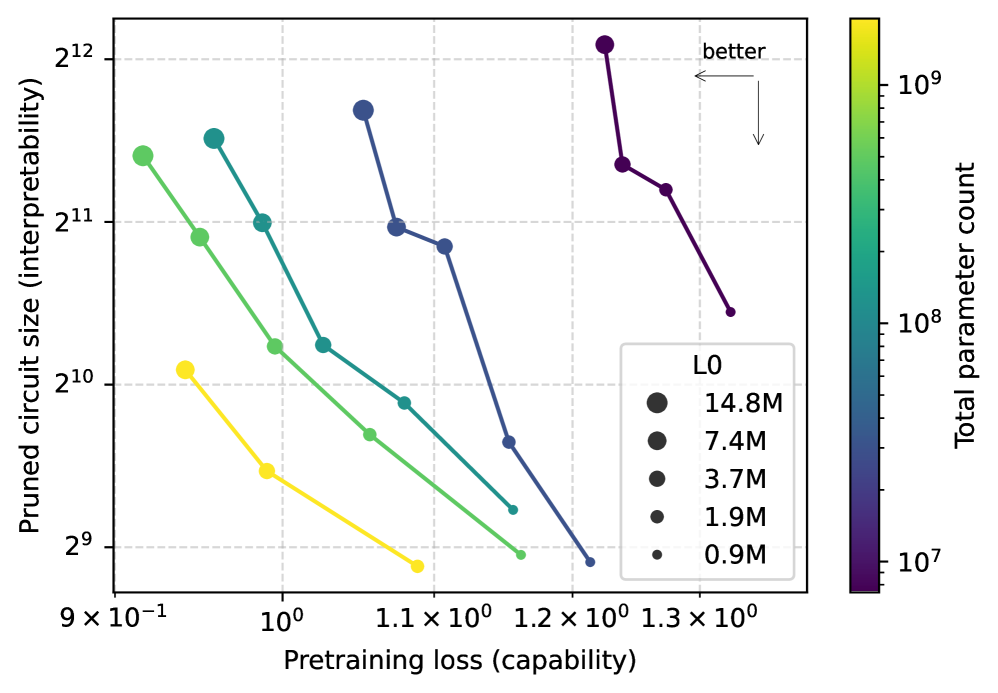
\includegraphics[width=0.8\textwidth]{images/scalingParams.png}
    \caption{The Interpretability-Capability Frontier. This visualization demonstrates how increasing model width improves performance at fixed sparsity levels. Reproduced from \autocite{gao2025weightsparsetransformersinterpretablecircuits}}
    \label{fig:depth}
\end{figure}


\begin{figure}[ht]
    \centering
    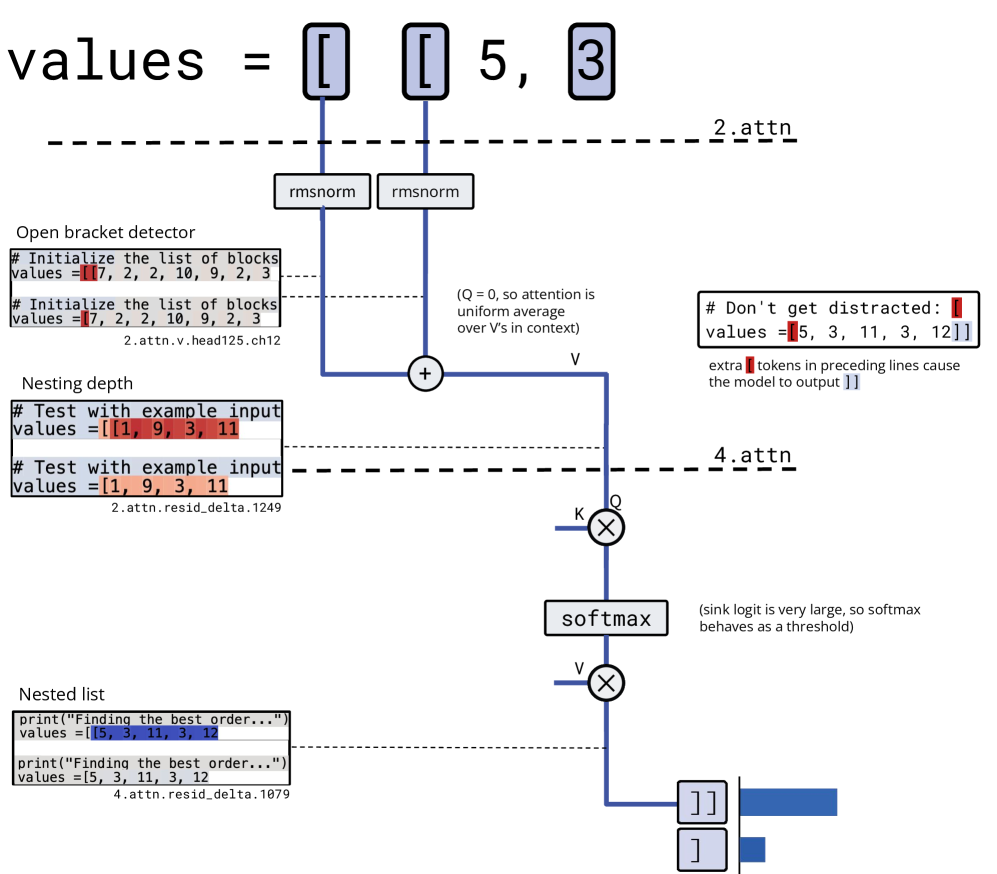
\includegraphics[width=0.8\textwidth]{images/x5.png}
    \caption{Simple illustration of the circuit for counting nesting depth. The attention head then averages the value of this detector over the context and writes it to the residual stream at each token (the “nesting depth”). A subsequent attention head reads out the nesting depth using a query channel, and thresholds it to only activate inside nested lists. This circuit uses 7 nodes and 4 edges. Understanding this algorithm allows us to adversarially attack the model with “distractors.”
    Reproduced from \autocite{gao2025weightsparsetransformersinterpretablecircuits}}
    \label{fig:sparse_frontier}
\end{figure}

\subsection{The Bracket-Closing Circuit}

One of the most compelling validations of this methodology is the discovery of the "Bracket-Closing" circuit. In standard dense models, predicting a closing bracket involves the integrated signal of thousands of infinitesimal weights. In the weight-sparse Transformer, this operation is distilled into a direct mechanism. By inspecting the non-zero entries in the $W_{OV}$ (Output-Value) and $W_{QK}$ (Query-Key) matrices, a specific attention head in the second layer was found that acts as a dedicated "Bracket Seeker". The sparse weights directly map the token for an open bracket to its corresponding closing pair. Sparse weights allow to verify the model’s logic simply by reading the weight matrix. \par
This simple circuit was not resistant towards easy traps as having a comment with an opening bracket one line above introduced this token for a bracket, thus the model wrongly predicted the number of closing brackets \autoref{fig:depth}. Similarly to this problem even dense counterparts can suffer from loosing the bracket attention when a list is too long, as the attention is taken over all the tokens.




\subsection{Bridges}

Activation Bridge mechanism was tested for its ability to interpret legacy dense models. By training a sparse proxy layer to mirror the activations of a dense GPT-2 model ~\cite{radford2019language} , the "induction head" within the dense model that had previously eluded detection. The bridge successfully recovered parts of the dense model’s logits, demonstrating that weight-sparse models can serve as a interpretation tool for dense models. This, of course, is limited by hardware and task complexity. 




\section{Conclusion}
\label{sec:conclusion}

This study aims to remove the "black-box" nature of Large Language Models. By moving away from post-hoc interpretability—which attempts to force explanations onto already complex dense models—and toward a framework of "interpretability by design". The weight-sparse transformer architecture provides a robust middle ground, achieving competitive cross-entropy losses on semi-complex datasets like Python code while maintaining a structural simplicity that allows for direct manual inspection. Through the exploration of the Interpretability-Capability Frontier, the methodology proves that with sufficient architectural width, a model can successfully disentangle its internal representations. This suggests that the difficulty in interpreting modern transformer architectures is not an inherent property of high-dimensional intelligence, but rather a byproduct of the dense parameter packing favored by current optimization standards. \par

The requirement of high dimensional matrices works in theory but still leaves a lot of dead neurons which still have to occupy space in memory, thus significantly worsening efficiency of these models. One possible solution would be to adapt the computations to adapt to the highly sparse design of the models by going around these dead neurons. \par
The attempt to retrieve interpretable circuits from dense model (GPT-2 ~\cite{radford2019language}) was successful for concrete binary tasks like predicting whether a string should end with a single or a double quote. Sparse model circuits are roughly 16-fold smaller (in terms of edge count) than those in dense models of comparable performance. The discovery of highly faithful circuits with minimal node counts provides a toolkit for AI safety and alignment. Researchers have a reliable pipeline to audit specific model behaviors, such as syntax tracking or logical induction, at a granular level. This has profound implications for the deployment of AI in high-stakes environments where approximate understanding is insufficient. By isolating these circuits, we can begin to build "verified" models where the causal paths from input to output are documented and understood. As we scale toward increasingly powerful systems, the ability to "read" a model’s weights as one would read source code will become a standard for trust and safety. Future work will likely focus on scaling these sparse constraints to billion-parameter models and exploring whether the same mechanistic clarity can be achieved in more abstract domains, such as natural language reasoning and creative synthesis.


%% 
%%%%%%%%%%%%%%%%%%%%%%%%%%%%%%%%%%%%%%%%%%%%%%%%%%%%%%%%%%%%%%%%%%%%%%%%%%%%%%%%

%%%%%%%%%%%%%%%%%%%%%%%%%%%%%%%%%%%%%%%%%%%%%%%%%%%%%%%%%%%%%%%%%%%%%%%%%%%%%%%%
%% 
%% Print the bibliography
%% 
%% (Optionally) let the bibliography start on a new odd page (odd is only relevant in twoside layout)
%\cleardoubleoddpage
\printbibliography
%% 
%%%%%%%%%%%%%%%%%%%%%%%%%%%%%%%%%%%%%%%%%%%%%%%%%%%%%%%%%%%%%%%%%%%%%%%%%%%%%%%%

%% Begin with the appendix part (all further sections will be appendices)
\appendix

%%%%%%%%%%%%%%%%%%%%%%%%%%%%%%%%%%%%%%%%%%%%%%%%%%%%%%%%%%%%%%%%%%%%%%%%%%%%%%%%
%% 
%% Add your appendix sections ...
%% 

%% Make sure to start the appendix on a new odd page (odd is only relevant in twoside layout)
%\cleardoubleoddpage
% \section{An Appendix}
% \label{app:an-appendix}

% Space for an appendix.
% You can have more than one appendix section.
% Appendices are, of course, optional.


% %% 
%%%%%%%%%%%%%%%%%%%%%%%%%%%%%%%%%%%%%%%%%%%%%%%%%%%%%%%%%%%%%%%%%%%%%%%%%%%%%%%%

\cleardoubleoddpage

\end{document}
\endinput
